\documentclass[spanish,12pt,letterpaper]{article}
\usepackage[a4paper, margin=2cm]{geometry}
\usepackage[T1]{fontenc}
\usepackage{graphicx}
\usepackage{enumitem}
\usepackage{float}
\usepackage[spanish]{babel}

\title{Doom Eternal}
\author{Cristian Guillermo Mejia Cisneros}
\date{\today}

\begin{document}
	\maketitle
	\newpage
	
	
	
	\section{¿Qué es Doom Eternal?}

    \subsection{Breve contexto}

   \noindent Doom Eternal, es un videojuego FPS (First Person Shooter) desarrollado por la empresa \textbf{id Software} y lanzado el 20 de marzo de 2020. Es continuación directa del \textbf{Doom (2016)} y secuela de la saga Doom en general.

    \subsection{Sinopsis}
    
	\noindent El juego esta ambientado años después de lo acontecido en \textbf{Doom (2016)}, después de haber sido encerrado por \textbf{Samuel Hayden}, el presidente de la \textit{Union Aerospace Corporation (UAC)} empresa creadora de los portales caracteristicos de la saga, Doom va en camino hacia la Tierra, con ayuda de su nave \textit{La fortaleza del destino} con el objetivo de acabar con las fuerzas demoníacas que han invadido el planeta. \\[1mm]


\section{Resumen del Lore del juego}

\subsection{Centinelas de la Noche}

\noindent Para comenzar a entender DOOM, debemos comenzar con los \textbf{Centinelas de la noche}, que son guerreros de un planeta llamado Argent, distinto a la tierra en el universo de DOOM (UD), que combaten a las fuerzas demoníacas desde hace millones de años con ayuda de seres divinos, los \textbf{Makyr}, que son los \textit{ángeles} en el \textbf{UD}, en particular sirven a un ángel en particular, llamada la \textit{Khan Makyr}.

\subsection{Sacerdotes del infierno}

\noindent Dentro del \textbf{UD}, de manera muy resumida, son seres ancestrales que anteriormente servían a los \textbf{centinelas de la noche}, pero que fueron corrompidos por las fuerzas demoníacas y organizaron el ataque a la tierra.

\subsection{Doom 64}

\noindent Durante el videojuego \textbf{Doom 64}, el DoomGuy (protagonista de la saga Doom), pelea contra los demonios debido a una invasión a la tierra ocurrida por culpa de los portales creados por la \textbf{UAC}, esta tierra es la de la linea del tiempo original del DoomGuy, distinta de alguna manera a la tierra de \textbf{Doom Eternal}. \\[1mm]

\noindent DoomGuy, cansado de tantas invasiones decide quedarse a vivir en el infierno de forma permanente con el proposito de combatir a los demonios hasta el fin de sus tiempos. \\[1mm]

\noindent Debido a la masacre brutal que el DoomGuy estaba cometiendo en el infierno, la \textbf{Madre Demonio}, líder de los demonios en ese momento, utiliza sus fuerzas para desterrar al DoomGuy a una linea temporal y universo distinto al que se encuentran, lo anterior, termina provocando que termine varado en el planeta Argent.

\subsection{Doom y los centinelas de la noche}

\noindent Los centinelas terminan encontrando a DoomGuy y lo llevan a un arena de batalla donde llevan a todos los capturados, y los hacen pelear entre si, quien termina victorioso en este pelea, tiene el derecho de seguir viviendo. En este lugar el DoomGuy termina derrotando a todos, repitiendo de manera insistente \textit{Destrozar y desgarrar} después de la batalla, denotando su estado mental deteriorado y pensando únicamente en eliminar demonios. Los sacerdotes informan sobre esto a la Khan Makyr, que llama su atención y terminan entrena dolo como a cualquier otro centinela, donde se dan cuenta que es un ser especial, alguien que puede enfrentarse a los demonios, que no les tiene miedo, el arma definitiva.

\subsection{Samur Makyr y la maquina de divinidad}

\noindent \textbf{Samur Makyr} es un ser de la raza Makyr y con el grado de Serafin entre su raza, no hay mucho que agregar de el, pero el hecho de mencionarlo es que el termina convirtiendo en un semidios a DOOM cuando lo introduce dentro de un dispositivo llamado \textit{la máquina de la divinidad}.\\[1mm]

\noindent Está maquina es un dispositivo que convierte, a cualquier ser que lo resiste, en un ser incorruptible, con una voluntad fuera de lo humano, fuerzas y capacidad asombrosas, así como el hecho de ser prácticamente inmortal; Samur al notar el don que el DoomGuy posee algo distinto a cualquiera, lo somete a esta máquina, convirtiéndolo en el arma definitiva, que termina destruyendo a cualquier demonio a su paso, provocando que los demonios por fin temieran a algo, al DoomGuy, creando incluso un códice con todas las leyendas de terror que se contaban de el y terminaron llamándolo el Slayer.

\subsection{Doom (2016)}

\noindent En unas de las peleas contra infierno que el DoomSlayer y los centinelas de la noche tenían, estos últimos fueron traicionados por otro centinela y terminaron emboscados por las fuerzas del infierno, todos perecieron a excepción del Slayer, que lucho durante eones de años sin ser abatido. Los demonios, llenos de miedo y sin casi opciones, encontraron que la única forma de detener al slayer, era sellándolo, pues incluso si lo mataban, podía regresar a la vida, así que engañándolo, fue encerrado en un sarcófago con la marca del Slayer, como símbolo de nunca abrir este sarcófago. \\[1mm]

\noindent Durante los sucesos de \textbf{Doom (2016)}, por alguna razón, Samuel Hayden, terminando encontrando el sarcófago y liberando al Slayer el cual perdio mucha de sus memorias pasadas, pero teniendo ciertos flashbacks. En este juego DoomSlayer derrota a varias fuerzas del infierno que querían atacar la tierra, y consigue un arma poderosa llamada el crisol. Samuel Hayden lo traciona teletransportandolo a otro lado y quitandole el crisol.

\subsection{Doom Eternal}

\noindent DoomSlayer llega a la tierra y se entera que los sacerdotes del infierno organizaron la invasión a demoniaca, esto con el hecho de matar a las personas y conseguir su alma, ya que, la razón por la que los demonios se interesan tanto en invadir planetas, es porque cuando torturan las almas de los seres vivos matados, estas liberan energía que alimenta a su planeta, en este sentido descubrimos que los demonios y ángeles, son seres de otros universos, más que fuerzas divinas. \\[1mm]

\noindent El Slayer termina derrotando a casi todos los demonios con el arsenal de armas que va encontrando durante su camino el cual es el siguiente:


\begin{itemize}
    \item Escopeta de combate
    \item Motosierra
    \item Cañón pesado
    \item Granadas de fragmentación
    \item Escupellamas
    \item Fusil de plasma
    \item Bombas de hielo
    \item Lanzamisiles
    \item Superescopeta
    \item Balista
    \item Ametralladora Gatling
    \item BFG-9000
    \item Crisol
    \item Desmakyr
\end{itemize}

\noindent Conforme avanza el juego, descubrimos que quien esta verdaderamente detrás de todo esto, es el angel Khan Makyr, los ángeles en realidad siempre estuvieron de lado de los demonios, ya que estos últimos compartían energía con los Makyr. Esto enfurece aún más al Slayer, pues tanto los centinelas como el han sido engañados durante bastante tiempo, por lo que termina asesinando a este ser, provocando el enojo de algo aun más poderoso...\\[1mm]

\noindent Al final DoomSlayer termina acabando con la invasión demoníaca, pero con la decisión de acabar con ella de manera en que los demonios no vuelvan a existir, busca una manera de borrar de la existencia del universo a los demonios de una ves y para siempre.

\section{Conclusión}

\noindent El documento escrito anteriormente es una muy breve explicación del Lore de Doom Eternal, donde se dejan muchas cosas ambiguas al azar, pero que no se explican con detalle pues no es el propósito además de no extender más las páginas, si hay interés en este videojuego, recomendamos enteramente jugarlo, pues es uno de los mejores FPS del siglo. Concluimos con una imagen del DoomSlayer:

\begin{figure}[H]
		\centering
		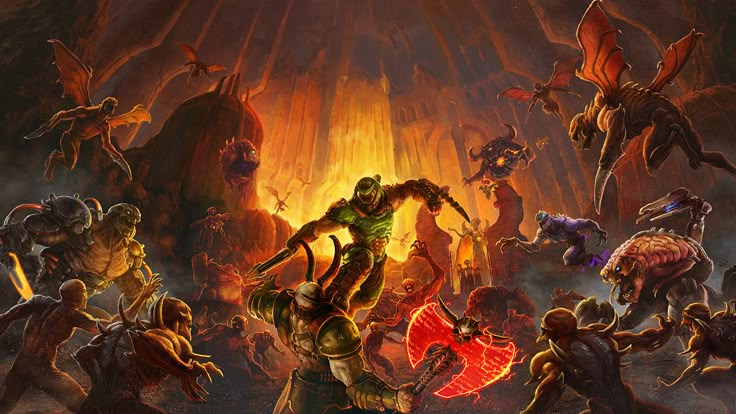
\includegraphics[width=0.7\textwidth]{Slayer.jpg}
		\caption{\textbf{DOOM Slayer}.}
	\end{figure}


\end{document}
